\documentclass[../sparc.tex]{subfiles}
\graphicspath{{\subfix{../images/}}}
\begin{document}

%%%%%%%%%%%%%%%%%%%%%%%%%%%%%%%%%%%%%%%%%%%%%%%%%%%%%%%%%%%%%%%%%%%%%%%%%%%%%%%%
\section{Wavelength}

\begin{figure}[ht]
  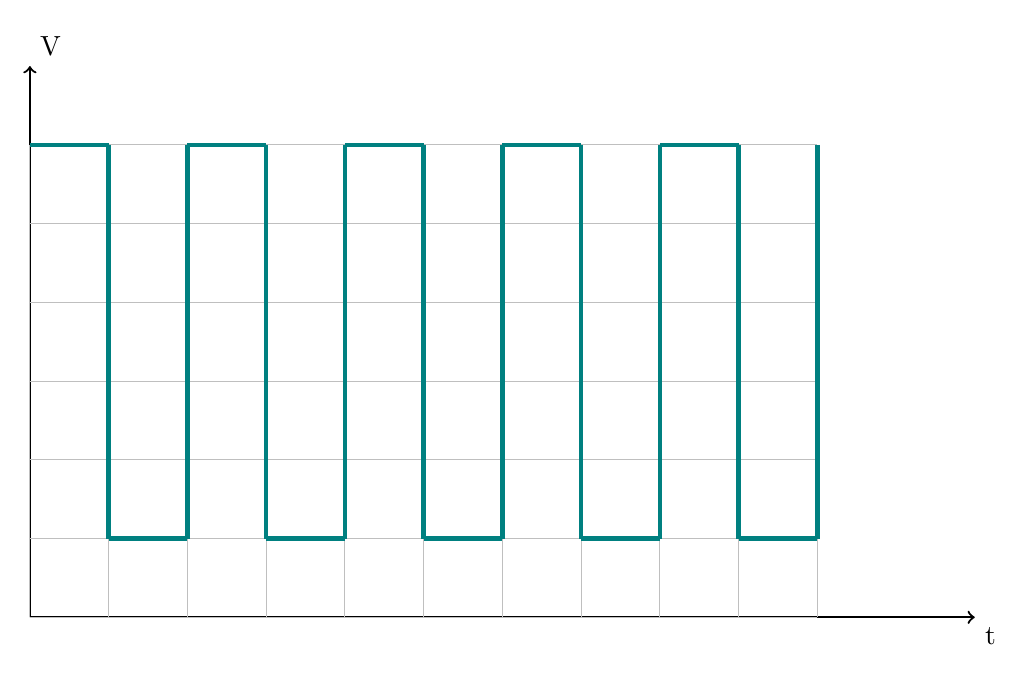
\begin{tikzpicture}
    \draw[thick, ->] (0, 0) -- (12, 0) node[anchor=north west] {t};
    \draw[thick, ->] (0, 0) -- (0,  7) node[anchor=south west] {V};
    \draw[lightgray] (0, 0) grid (10, 6);
    \foreach \x in {0, 2, ..., 8} {
      \draw[ultra thick, teal] (\x, 6) -- (\x + 1, 6);
      \draw[ultra thick, teal] (\x + 1, 6) -- (\x + 1, 1);
      \draw[ultra thick, teal] (\x + 1, 1) -- (\x + 2, 1);
      \draw[ultra thick, teal] (\x + 2, 1) -- (\x + 2, 6);
    }
  \end{tikzpicture}
  \caption{Graphical representation of a signal in relation to the time on a
    digital port.}
  \label{fig:blinking-led-graph}
\end{figure}

When we programmed our ``blinking lights'' project, we supplied to a digital
port signals \texttt{HIGH} and \texttt{LOW} alternately, with a delay specified
in microseconds.  If we take a look on the signal value in relation to the time
on a digital port (e.g. using an oscilloscope) we will get a graph similar to
fig. \ref{fig:blinking-led-graph}.

Where \emph{period length} is the distance between the two adjacent points in
time, where oscillations occur in the same phase.  If we know the period length
we can calculate the \emph{oscillation frequency}, and vice versa -- if we know
the frequency we can calculate the wavelength.

When we are working with \gls{PWM} we will be using the period length set in
microseconds ($\mu\mbox{s}$.)  1 microseconds is one millionth of a second.  For
the sake of brevity, we will be writing such small quantities of time in
scientific notation: that is, using powers of 10.  The table
\ref{table:timescale-units} shows various second fractions.  \footnote{The full
list of multiplies and sub-multiplies can be found in the article
\href{https://en.wikipedia.org/wiki/Second}{``Second''} in Wikipedia.}

\begin{table}[H]
  \begin{tabular}{p{3cm}|p{4cm}|p{3cm}}
    Unit & Relation the second & Examples \\
    \hline \hline
    Second ($s$)
    & $ 1 \mbox{s} $ or $ 10^0 \mbox{s} $
    & $ 500 * 10^{0} = 500 \mbox{s} $ \\
    \hline
    Millisecond ($\mbox{ms}$)
    & $ 0.001 \mbox{s} $ or $ 10^{-3} \mbox{s} $
    & $ 500 * 10^{-3} = 500 \mbox{ms} $ \\
    \hline
    Microsecond ($\mu\mbox{s}$ or just ``us'')
    & $ 0.000001 \mbox{s} $ or $ 10^{-6} \mbox{s} $
    & $ 500 * 10^{-6} = 500 \mu\mbox{s} $ \\
    \hline
    Nanosecond ($\mbox{ns}$)
    & $ 0.000000001 \mbox{s} $ or $ 10^{-9} \mbox{s} $
    & $ 500 * 10^{-9} = 500 \mbox{ns} $
  \end{tabular}
  \caption{Units of time measurement.}
  \label{table:timescale-units}
\end{table}

\end{document}
